\section{Introduction} 

One of the major causes of cancer-related fatalities worldwide, liver cancer, is becoming more common. For an appropriate liver cancer diagnosis and therapy, tumor areas in histopathology images must be precisely identified and segmented. On the other hand, pathologists must manually segment samples, which takes time and is prone to inter-observer variability. These restrictions can be overcome by automated segmentation of liver histopathology images, which enables quicker and more reliable tumor region segmentation. Due to recent developments in deep learning approaches, there has been a rise in interest in creating automated segmentation algorithms for liver histopathology images. These techniques can support the development of personalized medicine approaches as well as the precise and effective interpretation of large-scale histopathology image data.


Continuous progress had been made in the segmentation tasks. Cirasen et al. \cite{ciresan2012deep} propose a deep learning approach using a convolutional neural network to segment neuronal membranes in electron microscopy images. For segmentation, they use a pixel-by-pixel sliding window approach. This method is time-consuming, so Long et al. \cite{shelhamer2016fully} fully proposed the use of fully convolutional neural networks for image segmentation tasks, eliminating the need for fully connected layers and enabling end-to-end training. On the PASCAL VOC 2012 dataset, the proposed architecture achieved state-of-the-art semantic segmentation performance.
SegNet \cite{badrinarayanan2015segnet} was introduced, which uses an encoder-decoder architecture with skip connections to perform semantic segmentation of images. They show SegNet's performance on a variety of benchmark datasets, as well as its ability to produce accurate segmentation results while remaining computationally efficient. Unet architecture \cite{DBLP:journals/corr/RonnebergerFB15} was a significant breakthrough because of its accuracy in segmenting biological cells. It captures context using a contracting path and pinpoints precise localization using a symmetric expanding path.
The architectural style has been widely used in various medical image segmentation tasks, with promising results. Because it is particularly effective when dealing with limited training data, the U-Net is a popular choice in the field of medical image analysis. Chanchal et al. \cite{chanchal2021efficient} developed a model that uses the hypercolumn technique and the spatial convolution pyramidal pooling (SCPP) block to capture fine image details across multiple layers of pooling stages. This aided them in achieving better segmentation results. In another recent paper, \cite{chanchal2022deep} proposed the DRESDEN model using deapthwise separable convolution and residual connections within the encoder and decoder. This has resulted in cutting-edge results in histopathology-based image segmentation tasks.

Our research on segmentation tasks was in its primary stages. Still, we were able to experiment and draw conclusions that could be used as benchmarks for the next batch.

\section{Dataset}

For the experiment, a proprietary dataset of liver tissues obtained from KMC was used. This dataset includes 234 train and 5 test patches of liver tissue, as well as the appropriate segmentation masks. The original image size was 512x512; however, it was resized to 128x128 before being fed into the neural network. At the primary stage, no augmentation was performed. A sample image and its mask are shown as an example in Fig. \ref{Fig: Segmentation dataset example}

\begin{figure}[ht!]
\centering
\scalebox{1}{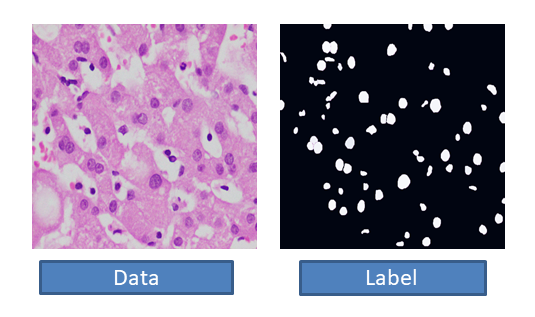
\includegraphics[width=3in]{Images/Dataset example.png}}
\caption{Segmentation dataset example}
\label{Fig: Segmentation dataset example}
\end{figure}


\section{Methodology}

We first intended to test a range of SOTA models on our dataset. We picked three distinct architectures for this experiment: Unet \cite{DBLP:journals/corr/RonnebergerFB15} MaNet \cite{fan2020ma} and Unet++ \cite{zhou2018unet++}. The models are imported from the SegmentationModels library. Image \ref{Fig: A general encoder decoder architecture} depicts a segmentation task architecture. The model, as indicated in the image, is made up of an encoder and a decoder. The encoder compresses the image while retrieving the critical information needed for segmentation. A steady deconvolution procedure in the decoder aids the rebuilt picture in acquiring suitable image characteristics.


\begin{figure}[ht!]
\centering
\scalebox{1}{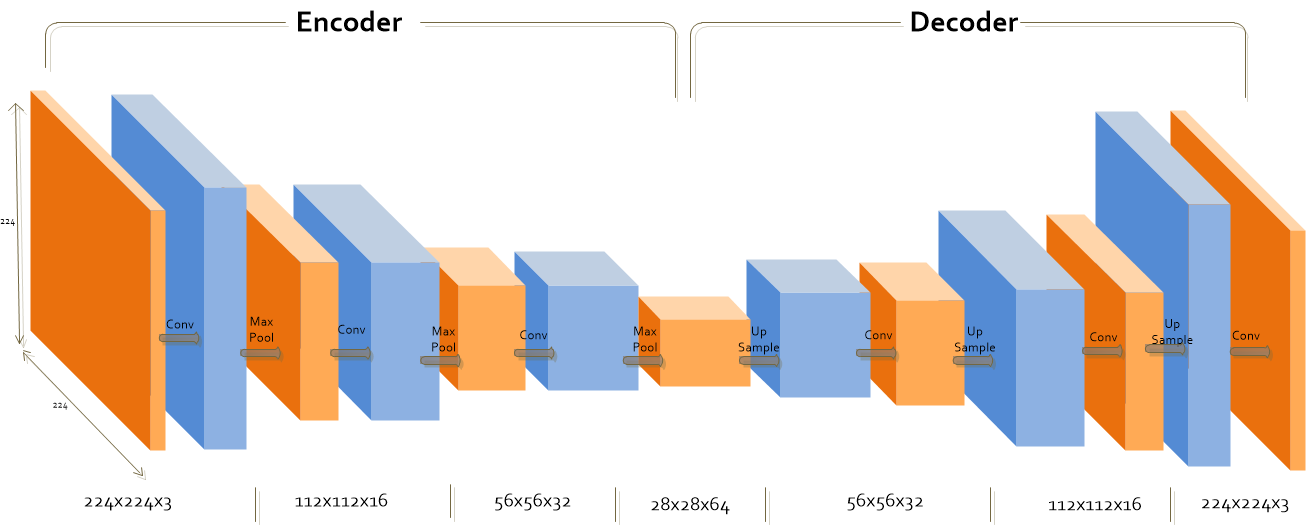
\includegraphics[width=3in]{Images/Drawing2.png}}
\caption{A general encoder decoder architecture}
\label{Fig: A general encoder decoder architecture}
\end{figure}

It was discovered that different encoders work better for different tasks. As a result, we investigated the performance of these designs with various encoders. EfficientNetb0, EfficientNetb1, EfficientNetb2, EfficientNetb3, EfficientNetb4, EfficientNetb5, EfficientNetb6, EfficientNetb7, EfficientNetb8, MobileNet v2. These models were trained for 35 epochs with a batch size of 16. As the cost function, binary cross-entropy loss was used in the Adam optimizer, and the initial learning rate was fixed at 0.001 with cosine annealing warm restarts every 12 epochs. Furthermore, to eliminate overfitting, a weight decay of 0.00001 was maintained. All three architectures were trained using 5-fold cross-validation and evaluated on the given dataset.

After training these models, the two top performers were chosen and finetuned to a particular depth. Experiments were conducted with a high level of fine tuning in order to improve model performance. Accuracy, F1-score, and intersection over union (IOU) were utilized as performance measurements.

\section{Results and Discussion}

Fig. \ref{Fig: Results of segmentation} shows the accuracy, F1-score, and IOU plots of all the architectures with varying encoders. The x axis shows the number of parameters available in the model. Circle, triangle, and MaNet represent Unet, Unet++, and MaNet architectures. Different colors are associated with different encoders. MaNet with the EfficientNetb0 backbone achieves 96.68\% accuracy, the lowest among all.
Unet++ with VGG16 backbone obtains the maximum accuracy of 98.13\%, while Unet with EfficientNetb0 backbone earns the lowest F1-Score of 96.23\%. Unet++ with VGG16 backbone earns 98.11\% F1-Score, which is the greatest among all, whereas Unet with EfficientNetb0 backbone achieves 93.77\% IOU, which is the lowest among all. Unet++ with a VGG16 backbone obtains the highest IOU of 96.53\% of all. Fig. \ref{Fig: acc vgg segmentation} shows the accuracy curve of the best-performing model.

\begin{figure}[ht!]
\centering
\scalebox{1}{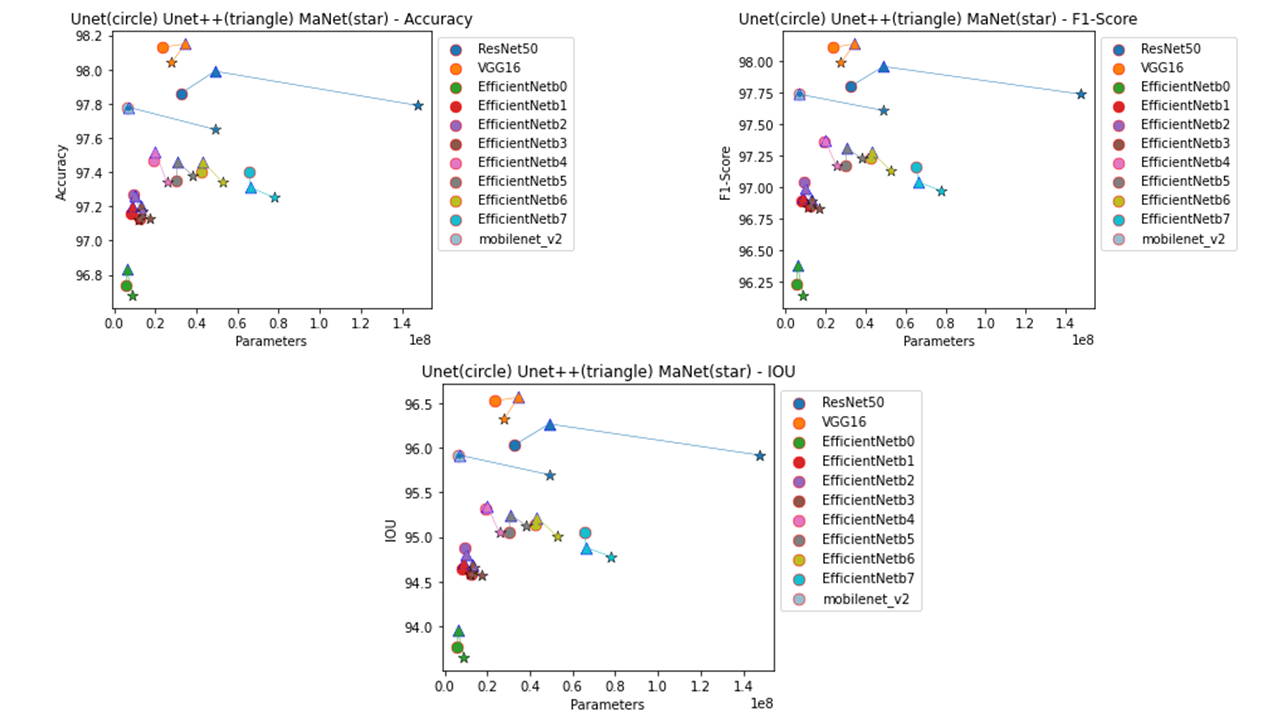
\includegraphics[width=6.5in]{Images/segmentation results.png}}
\caption{Figure shows accuracy, F1-score, and IOU of all the models. Circle, triangle, and MaNet represent Unet, Unet++, and MaNet architectures. Different colors are associated with different encoders.}
\label{Fig: Results of segmentation}
\end{figure}

\begin{figure}[ht!]
\centering
\scalebox{1}{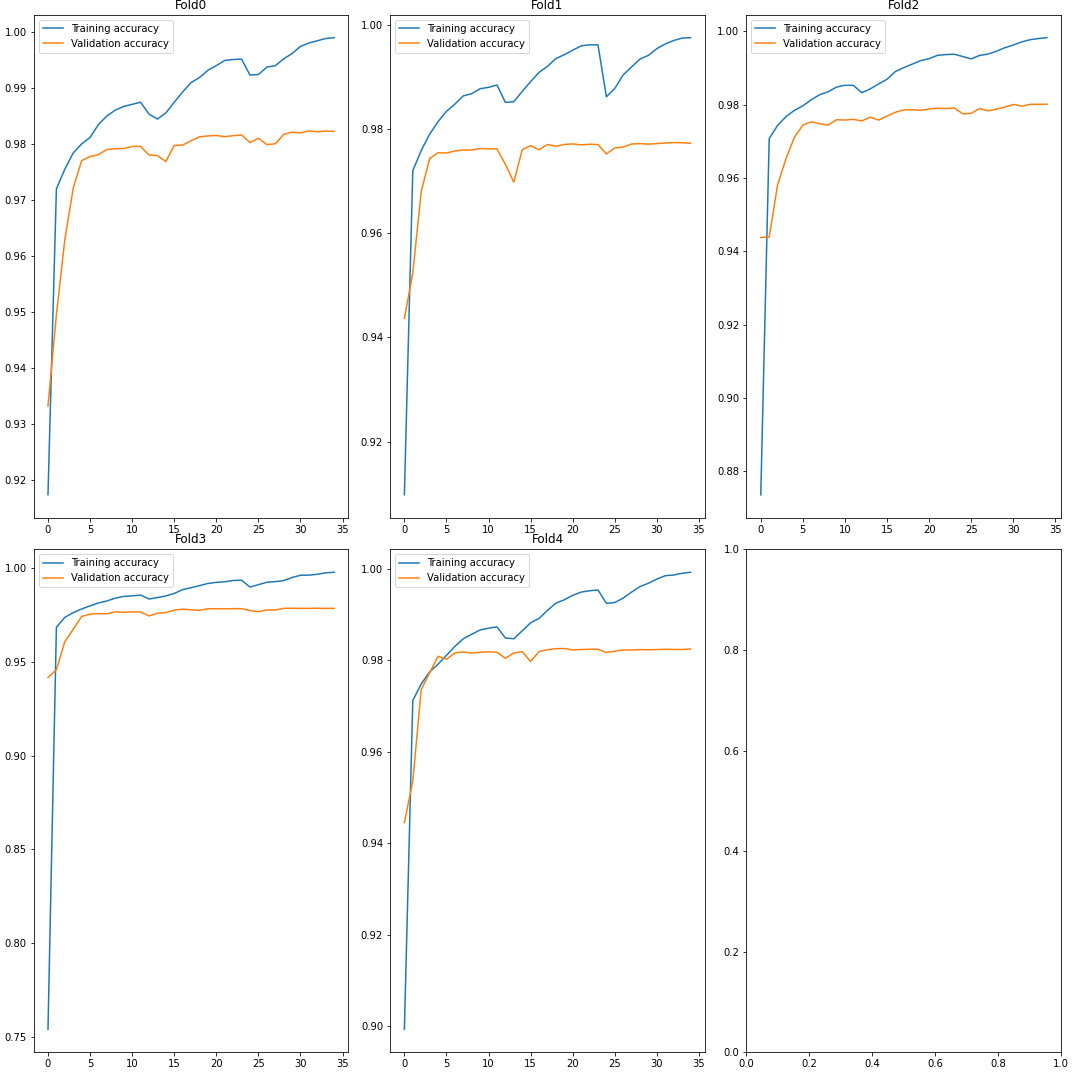
\includegraphics[width=4in, height=3.5in]{Images/Accuracy plot of vgg16 Unet++.png}}
\caption{Figure shows accuracy, Unet++ architecture having VGG16 as encoder}
\label{Fig: acc vgg segmentation}
\end{figure}


The results demonstrate that MaNet architectures are weak at extracting information and, consequently, cannot conduct appropriate segmentation. The MaNet architecture was discovered to overfit the train dataset as well.
EfficientNet takes a huge quantity of data to train well since it is a highly parameterized model architecture. Since the liver cancer dataset is small, VGG16's lower complexity and fewer parameters allow it to generalize better and outperform EfficientNet. EfficientNets demonstrate a steady improvement in accuracies across increament parameters, i.e., progression from B0 to B7 models, although this is still significantly lower than the VGG16 encoder.

Residual connections and model scaling are two interesting facts that might explain this behavior. Residual connections assist in retaining gradients but compromise the image's integrity by introducing high level information. Segmentation is an image-editing activity in which such residual connections behave like noise. VGG16 comprises just convolutional blocks and helps retain integrity; therefore, it may outperform the ResNet and EfficientNet models.

The obtained results were still unsatisfactory, as evidenced by accuracy plots of all folds of Unet++ with the VGG16 encoder, the highest performing model (Fig. \ref{Fig: acc vgg segmentation}). On the training dataset, the model appears to be overfitting. For finetuning, the two top performing models, Unet VGG16 and Unet ResNet, were chosen. The plot for performance metrics varying across the depth of finetuning is shown in Fig. \ref{Fig: fine tuning result}. The model performs best when all layers are unfrozen and finetuned, as seen in the figure. Note that the architectures were pre-trained using the ImageNet dataset. This indicates that pre-trained weights are useless for training. Furthermore, the accuracies do not differ significantly by varying the depth of fine tuning. The reason behind this overparameterization is discussed in Arora et al.'s study \cite{arora2018optimization}. The model has already learned what it can from the small amount of data available. Fine tuning does not lead to further improvement in performance.
\begin{figure}[ht!]
\centering
\scalebox{1}{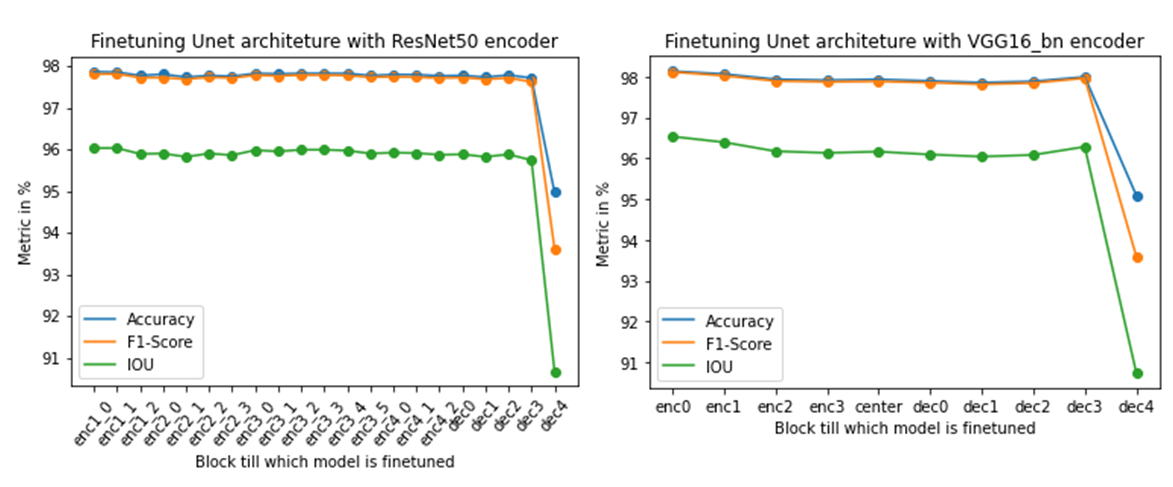
\includegraphics[width=5in]{Images/fine tuning result.png}}
\caption{Figure shows accuracy. F1-score, IOU of VGG16 and ResNet50 Unet architechtures varying over depth of finetuning}
\label{Fig: fine tuning result}
\end{figure}


As seen in Fig. \ref{Fig: Results example}, the predicted mask is pretty similar to the real one, but there appears to be a lot of room for improvement. In the future, various augmentation strategies, model tweaks, or other ways for improving segmentation model performance might be attempted. However, we see this as a difficult task that requires a significant amount of work.
\begin{figure}[ht!]
\centering
\scalebox{1}{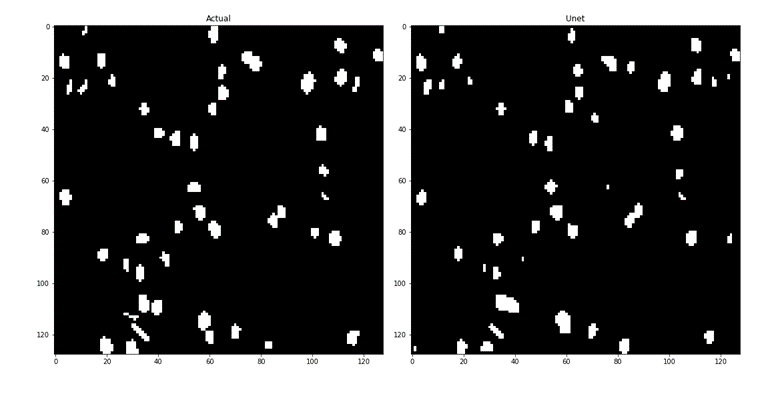
\includegraphics[width=4in]{Images/Results example.png}}
\caption{Figure shows actual and predicted masks of Unet architecture with VGG16 encoder}
\label{Fig: Results example}
\end{figure}

